\section{Versuchsaufbau und Messgeräte}
\subsection{AC-Suzeptibilität}
Für die Messung der AC-Suszeptibilität verwenden wir eine spezielle Schaltung, die sogenannte Hartshorn-Spulensystem. Dieses besteht aus einer Primärspule mit 2116 Windungen, welche von einem WEchselstrom durchflossen wird. Das von ihr erzeugte Magnetfeld induziert in zwei sekundärspulen mit der gleichen Windungszahl wiederum einen Strom, welcher sich aufgrund des entgegengesetzten Windungssinns im nachgeschalteten OPV und Spannungsmessgerät aufhebt. Der Aufbau ist in Abbildung \ref{aufbau-AC} nochmals dargestellt. Bringt man nun in eine der beiden Spulen ein magnetisches Material, ändert sich die Flussdichte in der entsprechenden Spulen und das Messignal ist ungleich null, welches von der Änderung der Magnetisierung mit dem Magnetfeld H, also von $\frac{\partial M}{\partial H}$ abhängt.


\begin{figure}[h!]
	\centering
	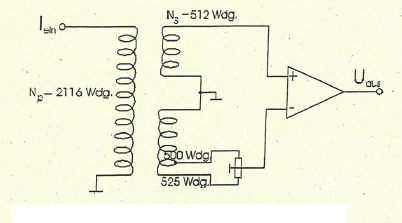
\includegraphics[height=8cm]{AC-auf.png}	
	~ %
	\caption{Hartshorn-Spulensystem für Messung der AC-Suszeptibilität \cite{Anleitung}}
	\label{aufbau-AC}
\end{figure}

\subsection{Phasenübergang der Indiumprobe}
Die Probe befindet sich auf einer Messapperatur in einem aufwändigen Kryostat mit fünf Glasschichten, die von außen nach Innen trennen: Luft ($T=300$K), Vakuum (thermische Isolation), Stickstoff ($T=75$K), Vakuum, Helium ($T=4,2$K), vgl. hierzu Abbildung \ref{aufbau}.

\begin{figure}[h!]
	\centering
	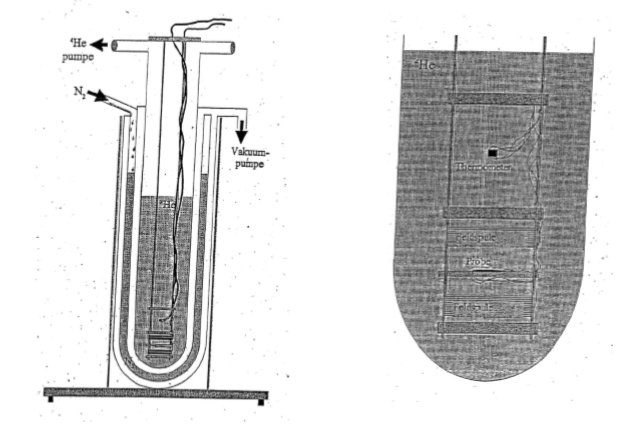
\includegraphics[height=8cm]{Aufbau.png}	
	~ %
	\caption{Messaufbau Phasenübergang Indium-Probe. \cite{Anleitung}}
	\label{aufbau}
\end{figure}

Für Indium gilt erfahrungsgemäß etwa $T_c=3,41$K, was sich unterhalb der Siedetemperatur von Helium befindet. In dem die Apperatur einem Unterdruck ausgesetzt wird, reduziert man die Temperatur (klassische Thermodynamik: Der Entzug der Verdampfungsenthalpie sorgt für eine Reduktion der Temperatur). Dadurch ist es möglich, durch bloßes Öffnen und Schließen der Ventile den Temperaturbereich von $T$=2 bis $T$=4K zu durchfahren. Währenddessen werden am Computer über einen Lock-In-Verstärker mit gespeicherter Eichkurve ständig Messwerte aufgenommen und direkt in ein R-T-Diagramm aufgetragen. Der Prozess geschieht hinreichend langsam, als dass das System im ständigen Gleichgewicht betrachtet werden kann.
